%%%%%%%%%%%%%%%%%%%%%%%%%%%%%%%%%%%%%%%%%%%%%%%%%%%%%%%%%%%%%%%%%%%%%%%%%%%%%%%%%%%%%%%%%%%%%%%%%%%%
%	chap02 (データの整理)
%===================================================================================================
%	AUTHOR	H. NAKAJIMA
%	DATE	2025/01
%===================================================================================================
%	EDIT HISTORY
%	DATE		NAME			OVERVIEW
%---------------------------------------------------------------------------------------------------
%	2025/01		H. NAKAJIMA		Create new
%%%%%%%%%%%%%%%%%%%%%%%%%%%%%%%%%%%%%%%%%%%%%%%%%%%%%%%%%%%%%%%%%%%%%%%%%%%%%%%%%%%%%%%%%%%%%%%%%%%%

{
	\centering
	{\textbf{第 2 章 \indent データの整理}} \\
}

{\textbf{\S 2.1 \indent 1 次元のデータ}}
\basic
\begin{qenumerate}
	\item{
		累積度数分布表は以下のようになる.
		\begin{table}[H]
			\centering
			\begin{tabular}{c|c|c} \hline
				階級値 (cm) & 累積度数 & 累積相対度数 \\ \hline
				164 &  5 & 0.125 \\
				168 & 13 & 0.325 \\
				172 & 25 & 0.625 \\
				176 & 31 & 0.775 \\
				180 & 36 & 0.900 \\
				184 & 40 & 1.000 \\ \hline
			\end{tabular}
		\end{table}
	}
	\item{
		ヒストグラムと度数折れ線は以下のようになる.
		\begin{figure}[H]
			\centering
			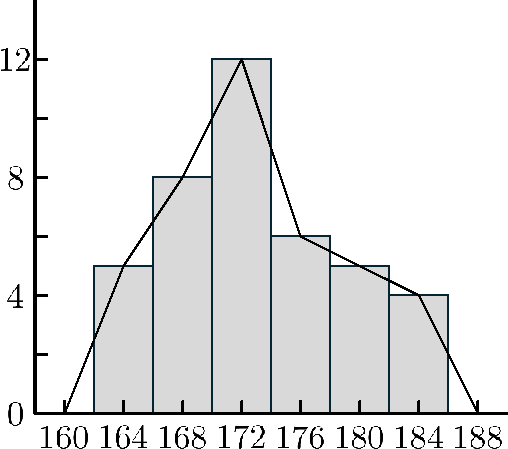
\includegraphics[scale = 0.5]{./figure/73.pdf}
		\end{figure}
	}
	\item{
		求める平均 $\overline{x}$ は
		\begin{align}
			\overline{x} &= \frac{5\cdot 164 \! + \! 8 \! \cdot \! 168 \! + \! 12 \! \cdot \! 172 \! + \! 6 \! \cdot \! 176 \! + \! 5 \! \cdot \! 180 \! + \! 4 \! \cdot \! 184}{40} \\
				&= \red{173}.
		\end{align}
	}
	\item{
		変換後のデータは
		\begin{align}
			u: \red{-12}, \quad \red{11}, \quad \red{-4}, \quad \red{15}, \quad \red{18}, \quad \red{-18}, \quad \red{16}
		\end{align}
		である.
		またデータの平均は, $\overline{u} = \dfrac{\overline{x} - 30}{0.01}$ より
		\begin{align}
			\overline{x} &= 0.01\overline{u} + 30 \\
				&= 0.01\cdot\frac{-12 \! + \! 11 \! + \! (-4) \! + \! 15 \! + \! 18 \! + \! (-18) \! + \! 16}{7} + 30 \\
				&\simeq 0.01\cdot 3.7 + 30 \\
				&\simeq \red{30.04}. 
		\end{align}
	}
	\item{
		\begin{enumerate}
			\item{
				平均値 $\overline{x}$ は
				\begin{align}
					\overline{x} = \frac{1 + 1 + 2 + 3 + 4 + 5 + 5 + 7 + 9 + 10}{10} = \red{4.7}.
				\end{align}
				データ数が偶数だから, 中央値は
				\begin{align}
					\frac{4 + 5}{2} = \red{4.5}.
				\end{align}
			}
			\item{
				平均値 $\overline{x}$ は
				\begin{align}
					\overline{x} = \frac{1 + 1 + 2 + 3 + 4 + 5 + 6 + 7 + 9 + 10 + 18}{11} = \red{6}.
				\end{align}
				データ数が奇数だから, 中央値は\red{5}.
			}
		\end{enumerate}
	}
	\item{
		度数が一番大きい階級は 60--65 だから, 最頻値は
		\begin{align}
			\frac{60 + 65}{2} = \red{62.5}.
		\end{align}
		データ数が 45 だから, 中央値は順に並んだデータの 23 番目のデータである.
		以下の累積度数分布表において, 累積度数が 23 になる階級は \red{55--60}.
		\begin{table}[H]
			\centering
			\begin{tabular}{c|c|c} \hline
				階級 (kg) & 度数 & 累積度数 \\ \hline
				40--45 &  2 &  2 \\
				45--50 &  4 &  6 \\
				50--55 & 12 & 18 \\
				\textbf{55--60} &  9 & \textbf{27} \\
				60--65 & 13 & 40 \\
				65--70 &  2 & 42 \\
				70--75 &  0 & 42 \\
				75--80 &  3 & 45 \\ \hline
			\end{tabular}
		\end{table}
	}
	\item{
		得点の最大値は 8, 最小値は 2 であるから, 範囲は $8 - 2 = \red{6}$.
		得点の平均 $\overline{x}$ は
		\begin{align}
			\overline{x} = \frac{4 + 6 + 2 + 8 + 3 + 6 + 5 + 3 + 6 + 7 + 5 + 8}{12} = \red{5.25}.
		\end{align}
		得点の分散 $v_{x}$ は
		\begin{align}
			v_{x} = \frac{(4 - 5.25)^{2} + \cdots + (8 - 5.25)^{2}}{12} \simeq 3.5208
		\end{align}
		であるから, 標準偏差 $s_{x}$ は
		\begin{align}
			s_{x} = \sqrt{v_{x}} = \sqrt{3.5208} = \red{1.876}.
		\end{align}
	}
	\item{
		気温の平均 $\overline{x}$ は
		\begin{align}
			\overline{x} &= \frac{19.6 + \cdots + 19.1}{10} = \red{20.65}.
		\end{align}
		気温の分散 $v_{x}$ は
		\begin{align}
			v_{x} = \frac{(19.6 - 20.65)^{2} + (19.1 - 20.65)^{2}}{10} = 7.8525
		\end{align}
		であるから, 標準偏差 $s_{x}$ は
		\begin{align}
			s_{x} = \sqrt{v_{x}} = \sqrt{7.8525} \simeq \red{2.802}.
		\end{align}
	}
	\item{
		女子学生の身長の平均 $\overline{x}$ は
		\begin{align}
			\overline{x} = \frac{4\cdot 146 + \cdots 2\cdot 174}{100} = \red{159.36}.
		\end{align}
		女子学生の身長の分散 $v_{x}$ は
		\begin{align}
			v_{x} = \frac{4\cdot (146 - 159.36)^{2} + 2\cdot (174 - 159.36)^{2}}{100} = 37.1904
		\end{align}
		であるから, 標準偏差 $s_{x}$ は
		\begin{align}
			s_{x} = \sqrt{v_{x}} = \sqrt{37.1904} \simeq \red{6.098}.
		\end{align}
	}
\end{qenumerate}

%\vspace{\baselineskip}
\check
\begin{qenumerate}
	\item{
		\begin{enumerate}
			\item{
				累積度数分布表は以下のようになる.
				\begin{table}[H]
					\centering
					\begin{tabular}{c|c|c} \hline
						階級値 (cm) & 累積度数 & 累積相対度数 \\ \hline
						157.5 &  1 & 0.025 \\
						162.5 &  6 & 0.150 \\
						167.5 & 17 & 0.425 \\
						172.5 & 31 & 0.775 \\
						177.5 & 38 & 0.950 \\
						182.5 & 40 & 1.000 \\ \hline
					\end{tabular}
				\end{table}
			}
			\item{
				ヒストグラムと度数折れ線は以下のようになる.
				\begin{figure}[H]
					\centering
					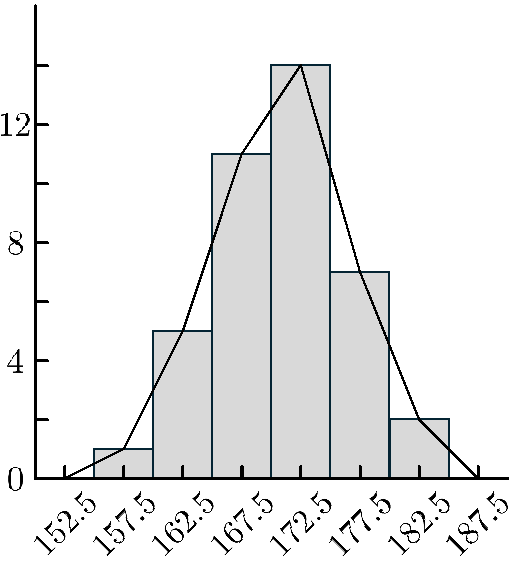
\includegraphics[scale = 0.5]{./figure/81.pdf}
				\end{figure}
			}
			\item{
				身長の平均 $\overline{x}$ は
				\begin{align}
					\overline{x} = \frac{1\cdot 157.5 + \cdots + 2\cdot 182.5}{40} = \red{170.9}.
				\end{align}
			}
		\end{enumerate}
	}
	\item{
		\begin{enumerate}
			\item{
				変量 $u$ のデータは
				\begin{align}
					u: \red{5}, \quad \red{2}, \quad \red{5}, \quad \red{4}, \quad \red{6}, \quad \red{5}, \quad \red{3}, \quad \red{2}
				\end{align}
				であり, これらの平均 $\overline{u}$ は
				\begin{align}
					\overline{u} = \frac{5 + 2 + 5 + 4 + 6 + 5 + 3 + 2}{8} = \red{4}.
				\end{align}
			}
			\item{
				鉛筆の重さの平均 $\overline{x}$ は, $\overline{u} = \dfrac{\overline{x} - 7.4}{0.01}$ より
				\begin{align}
					\overline{x} &= 0.01\overline{u} + 7.4 = 0.01\cdot 4 + 7.4 = \red{7.44}.
				\end{align}
			}
		\end{enumerate}
	}
	\item{
		\begin{enumerate}
			\item{
				台風の発生件数の平均 $\overline{x}$ は
				\begin{align}
					\overline{x} = \frac{21 + \cdots + 23}{10} = \red{26.1}.
				\end{align}
				また, データを昇順に並べると
				\begin{align}
					21\quad 23\quad 23\quad 25\quad 26\quad 27\quad 27\quad 29\quad 29\quad 31
				\end{align}
				となるから, 中央値は
				\begin{align}
					\frac{26 + 27}{2} = \red{26.5}.
				\end{align}
			}
			\item{
				(1) で昇順に並べたデータより, 範囲は $31 - 21 = \red{10}$.
				分散 $v_{x}$ は
				\begin{align}
					v_{x} = \frac{(21 - 26.1)^{2} + \cdot + (31 - 26.1)^{2}}{10} = \red{8.89}.
				\end{align}
				標準偏差 $s_{x}$ は
				\begin{align}
					s_{x} = \sqrt{v_{x}} = \sqrt{8.89} \simeq \red{2.982}.
				\end{align}
			}
		\end{enumerate}
	}
	\item{
		\begin{enumerate}
			\item{
				気温の平均 $\overline{x}$ は
				\begin{align}
					\overline{x} = \frac{5.3 + \cdots + 7.1}{12} \simeq \red{17.6}.
				\end{align}
				また, データを昇順に並べると
				\begin{align}
					&5.3\quad 7.1\quad 8.8\quad 10.6\quad 10.9\quad 16.3 \\
					&20.3\quad 22.8\quad 24.6\quad 26.8\quad 28.5\quad 29.1
				\end{align}
				となるから, 中央値は
				\begin{align}
					\frac{16.3 + 20.3}{2} = \red{18.3}.
				\end{align}
			}
			\item{
				(1) で昇順に並べたデータより, 範囲は $29.1 - 5.3 = \red{23.8}$.
				分散 $v_{x}$ は
				\begin{align}
					v_{x} = \frac{(5.3 - 17.6)^{2} + \cdot + (29.1 - 17.6)^{2}}{10} \simeq \red{71.13}.
				\end{align}
				標準偏差 $s_{x}$ は
				\begin{align}
					s_{x} = \sqrt{v_{x}} = \sqrt{71.13} \simeq \red{8.434}.
				\end{align}
			}
		\end{enumerate}
	}
	\item{
		\begin{enumerate}
			\item{
				度数が一番大きい階級は 170--175 だから, 最頻値は
				\begin{align}
					\frac{170 - 175}{2} = \red{172.5}.
				\end{align}
			}
			\item{
				データ数が 40 だから, 中央値は順に並んだデータの 20 番目のデータである.
				{\textbf{81}} (1) の累積度数分布において, 累積度数が 20 になる階級は \red{170--175}.
			}
			\item{
				{\textbf{81}} (3) より身長の平均は 170.9 だから, 身長の分散 $v_{x}$ は
				\begin{align}
					v_{x} &= \frac{1\cdot (157.5 - 170.9)^{2} + \cdots + 2\cdot (182.5 - 170.9)^{2}}{40} \\
						&\simeq \red{31.73}.
				\end{align}
				分散 $s_{x}$ は
				\begin{align}
					s_{x} = \sqrt{v_{x}} = \sqrt{31.73} \simeq \red{5.633}.
				\end{align}
			}
		\end{enumerate}
	}
	\item{
		通学時間の平均 $\overline{x}$ は
		\begin{align}
			\overline{x} &= \frac{1\cdot 5 + \cdots + 5\cdot 75}{80} \simeq \red{49.1}.
		\end{align}
		通学時間の分散 $v_{x}$ は
		\begin{align}
			v_{x} &= \frac{1\cdot (5 - 49.1)^{2} + \cdot + 5\cdot (75 - 49.1)^{2}}{80} = 211.735
		\end{align}
		であるから, 標準偏差 $s_{x}$ は
		\begin{align}
			s_{x} = \sqrt{v_{x}} = \sqrt{211.735} = \red{14.891}.
		\end{align}
	}
\end{qenumerate}

%\vspace{\baselineskip}
\stepup
\begin{qenumerate}
	\item{
		\begin{enumerate}
			\item{
				変量 $u$ のデータは
				\begin{align}
					u: \red{7}&, \quad \red{1}, \quad \red{3}, \quad \red{16}, \quad \red{8}, \quad \red{3}, \quad \red{10}, \quad \red{1}, \quad \red{11}, \\
						 \red{6}&, \quad \red{13}, \quad \red{5}, \quad \red{18}, \quad \red{16}, \quad \red{0}, \quad \red{11}, \quad \red{3}, \quad \red{9}
				\end{align}
				である.
			}
			\item{
				Sturges の公式より
				\begin{align}
					1 + \frac{\log{18}}{\log{2}} \simeq 5.17
				\end{align}
				となるから, 階級の数は 5 とする.
				また, 階級の幅はデータの範囲を階級の数で割って
				\begin{align}
					\frac{18 - 0}{5} = 3.6
				\end{align}
				となるから, 階級の幅は 4 とする.
				以上の条件から作られる度数分布表は以下のようになる.
				\begin{table}[H]
					\centering
					\begin{tabular}{c|c|c} \hline
						階級 & 階級値 & 度数 \\ \hline
						0 以上 4 未満   & 2 & 6 \\
						4 以上 8 未満   &  6 & 3 \\
						8 以上 12 未満  & 10 & 5 \\
						12 以上 16 未満 & 14 & 1 \\
						16 以上 20 未満 & 18 & 3 \\ \hline
						               & 計 & 18 \\ \hline
					\end{tabular}
				\end{table}
			}
			\item{
				ヒストグラムは以下のようになる.
				\begin{figure}[H]
					\centering
					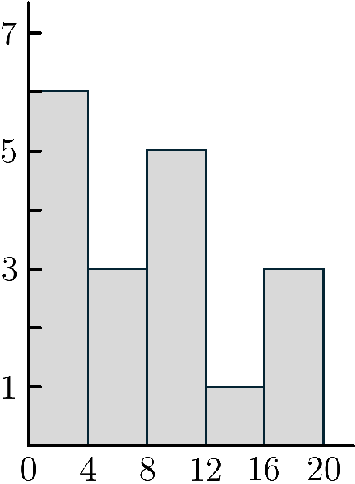
\includegraphics[scale = 0.5]{./figure/87.pdf}
				\end{figure}
			}
		\end{enumerate}
	}
	\item{
		5 歳の身長のデータを $x$, 17 歳の身長のデータを $y$ とすると, これらの平均 $\overline{x}$, $\overline{y}$ は
		\begin{gather}
			\overline{x} = \frac{115.5 + \cdots + 111.0}{10} = 110.19, \\
			\overline{y} = \frac{176.1 + \cdots + 170.6}{10} = 171.7
		\end{gather}
		である.
		また, これらの標準偏差 $s_{x}$, $s_{y}$ は
		\begin{align}
			s_{x} &= \sqrt{\frac{(115.5 - 110.19)^{2} + \cdots + (111.0 - 110.19)^{2}}{10}} \\
				&= \sqrt{12.6929} \simeq 3.563, \\
			s_{y} &= \sqrt{\frac{(176.1 - 171.7)^{2} + \cdots + (170.6 - 171.7)^{2}}{10}} \\
				&= \sqrt{17.2} \simeq 4.147
		\end{align}
		である.
		したがって, 5 歳の身長のデータの変動係数は
		\begin{align}
			\frac{s_{x}}{\overline{x}} = \frac{3.563}{110.19} \simeq \red{0.032}, 
		\end{align}
		17 歳の身長データの変動係数は
		\begin{align}
			\frac{s_{y}}{\overline{y}} = \frac{4.147}{171.7} \simeq \red{0.024}.
		\end{align}
	}
	\item{
		数学の得点のデータを $x$, 英語の得点のデータを $y$ とすると, これらの平均 $\overline{x}$, $\overline{y}$ は
		\begin{gather}
			\overline{x} = \frac{0\cdot 5 + \cdots + 0\cdot 95}{50} = 51.4, \\
			\overline{y} = \frac{0\cdot 5 + \cdots + 5\cdot 95}{50} = 64.6
		\end{gather}
		である.
		また, これらの標準偏差 $s_{x}$, $s_{y}$ は
		\begin{align}
			s_{x} &= \sqrt{\frac{0\cdot (5 - 51.4)^{2} + \cdots + 0\cdot (95 - 51.4)^{2}}{50}} \\
				&= \sqrt{255.04} \simeq 15.97, \\
			s_{y} &= \sqrt{\frac{0\cdot (5 - 64.6)^{2} + \cdots + 5\cdot (95 - 64.6)^{2}}{50}} \\
				&= \sqrt{283.84} \simeq 16.85
		\end{align}
		である.
		したがって, 数学の得点のデータの変動係数は
		\begin{align}
			\frac{s_{x}}{\overline{x}} = \frac{15.97}{51.4} \simeq \red{0.311}, 
		\end{align}
		英語の得点のデータの変動係数は
		\begin{align}
			\frac{s_{y}}{\overline{y}} = \frac{16.85}{64.6} \simeq \red{0.261}.
		\end{align}
	}
\end{qenumerate}